\documentclass{article}

% \usepackage{nips_2017}
\usepackage[final]{nips_2017}

\usepackage{polski}
\usepackage[utf8]{inputenc} % allow utf-8 input
\usepackage[T1]{fontenc}    % use 8-bit T1 fonts
\usepackage{hyperref}       % hyperlinks
\usepackage{url}            % simple URL typesetting
\usepackage{booktabs}       % professional-quality tables
\usepackage{amsfonts}       % blackboard math symbols
\usepackage{nicefrac}       % compact symbols for 1/2, etc.
\usepackage{microtype}      % microtypography
\usepackage[section]{placeins}
\usepackage{graphicx}
\usepackage{interval}

\title{Ćwiczenie 1 – proste sieci neuronowe} 
\author{Michał Kajstura}


\begin{document}

\maketitle

\begin{abstract}
 Celem ćwiczenia była implementacja dwóch prostych modeli neuronu.
 W pierwszym zadaniu zrealizowano model Perceptronu prostego, w drugim zaś
 model Adaline. Zbadano wpływ różnych parametrów na czas uczenia oraz porównano
 obie metody pod względem liczby epok potrzebnych do poprawnej klasyfikacji przypadków uczących. \href{https://github.com/michalkaj/sieci_neuronowe_7_sem}{Kod} potrzebny do przeprowadzania eksperymentów został napisany w języku Python.
\end{abstract}
\tableofcontents
\pagebreak

\section{Przygotowanie danych}
Na początku realizacji ćwiczenia wygenerowano zbiór syntetycznych danych 
imitujący funkcję logiczną AND.
Zbiór składał się ze 100 przykładów pozytywnych i negatywnych.
Do wyników funkcji dodano losowy szum o małej amplitudzie.

\begin{figure}[h]
  \caption{Wygenerowany zbiór danych}
  \centering
    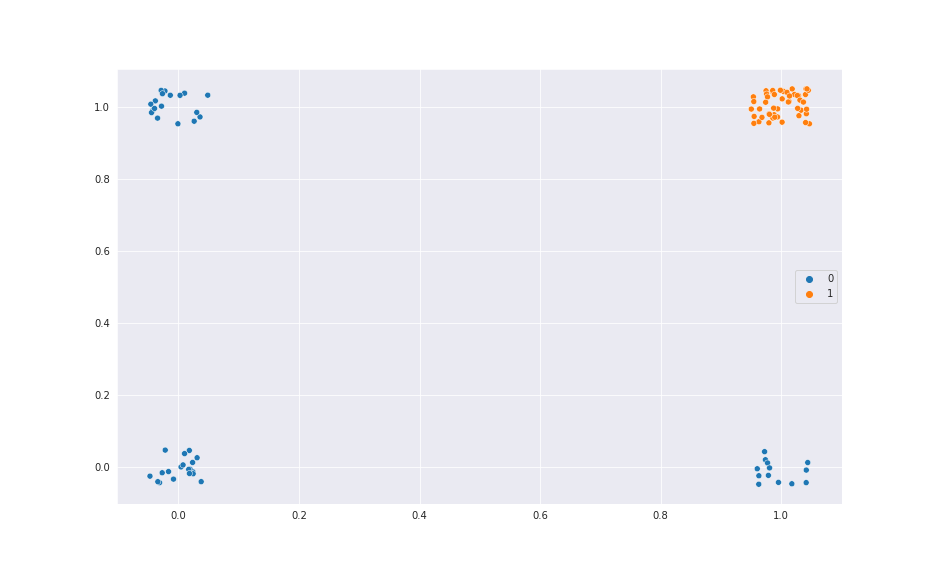
\includegraphics[width=0.8\textwidth]{images/01_data.png}
\end{figure}

\section{Badania}

\subsection{Metodyka badań}
Wszystkie eksperymenty powtórzono 20 razy dla każdej wartości badanego parametru.
Wyjątkiem jest badanie wpływu funkcji aktywacji, które wykonano 1000 razy, w celu
uzyskania bardziej miarodajnego wyniku. 

\pagebreak
\subsection{Perceptron}
\label{headings}

\subsubsection{Próg $\theta$}
Próg $\theta$ jest ważnym parametrem, który znacząco wpływa na szybkość uczenia.
Zarówno zbyt mała, jak i za duża wartość $\theta$ wpływa negatywnie na proces optymalizacji.
Wartości z przedziału $\left[0.01, 1\right]$ pozwalają wytrenować algorytm w stosunkowo krótkim czasie.

\begin{figure}[h]
  \caption{Wpływ parametru $\theta$}
  \centering
    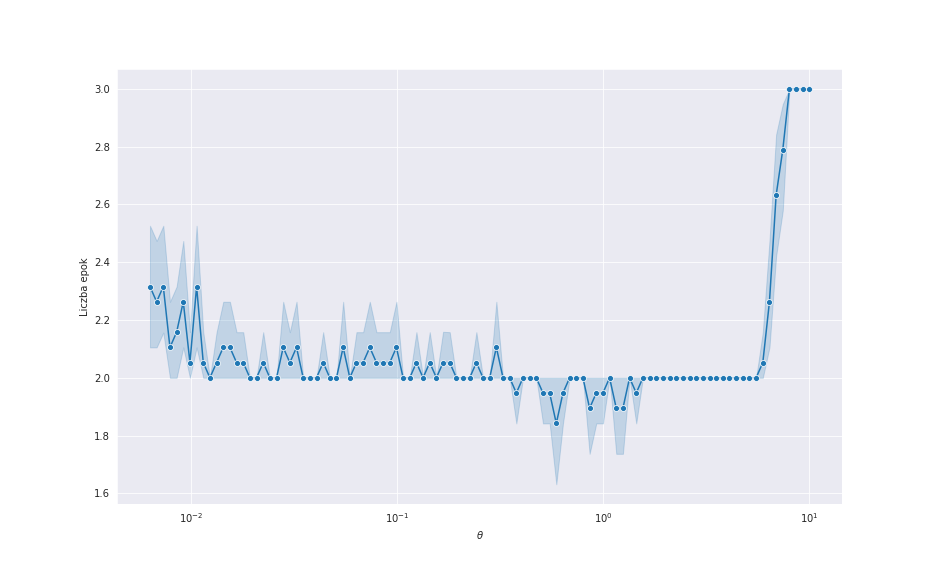
\includegraphics[width=0.8\textwidth]{images/02_per_theta.png}
\end{figure}

\FloatBarrier
\subsubsection{Inicjalizacja wag}

Wagi zostały zainicjowane z rozkłądu jednostajnego.
Na krańce przedziałów wybrano liczby leżące w tej samej odległości od puntu zerowego.
Wartości z przedziału $\left(0, 1\right]$ zapewniają najszybsze uczenie modelu.

\begin{figure}[h]
  \caption{Wpływ inicjalizacji wag}
  \centering
    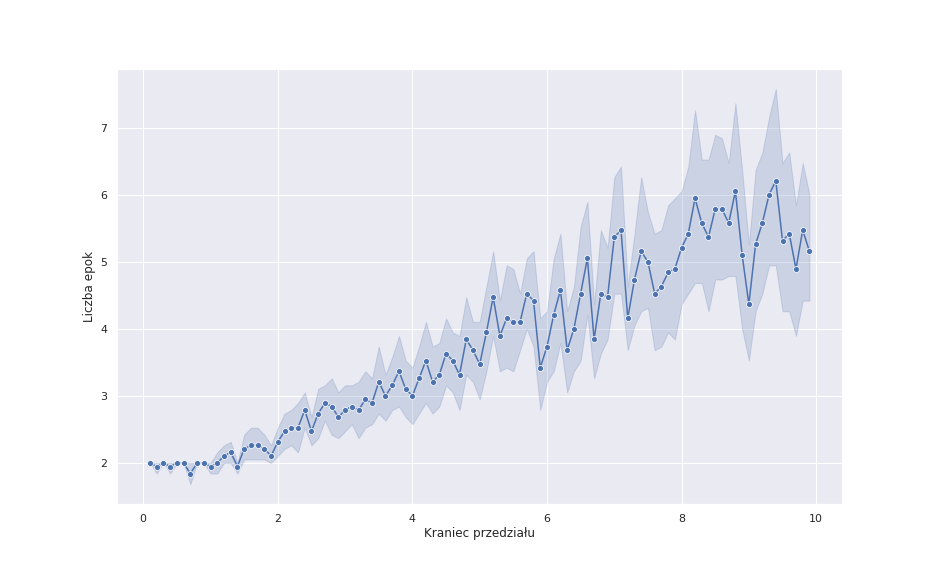
\includegraphics[width=0.8\textwidth]{images/03_per_interval.png}
\end{figure}

\FloatBarrier
\subsubsection{Współczynnik uczenia $\alpha$}
Hiperparametr $\alpha$ naturalnie wpływa na szybkość uczenia.
Zbyt małe wartości tego współczynnika skutkowały bardzo wolnym zbieganiem do optimum.
Co ciekawe, liczba epok pozostawała względnie stała dla większych wartości $\alpha$

\begin{figure}[h]
  \caption{Wpływ $\alpha$ }
  \centering
    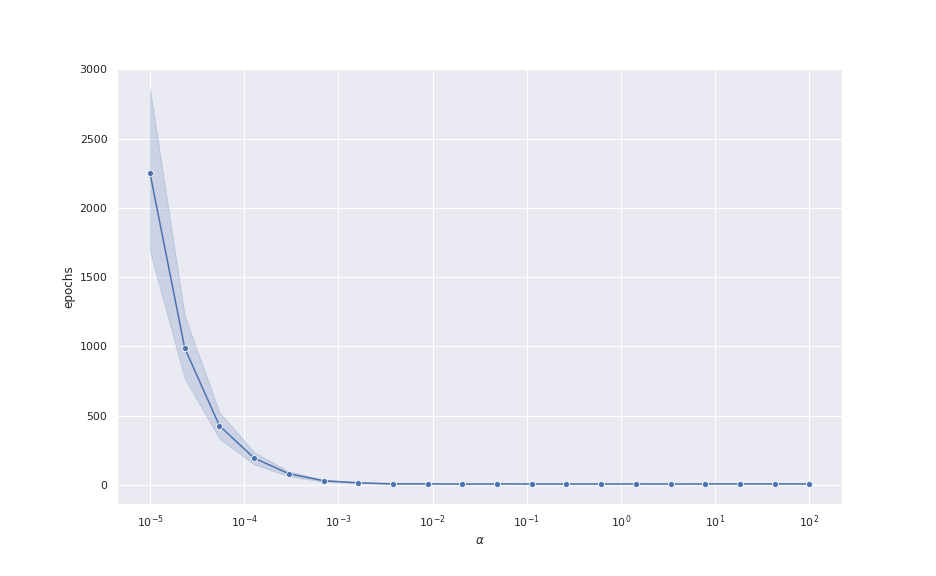
\includegraphics[width=0.8\textwidth]{images/04_per_lr.png}
\end{figure}

\FloatBarrier
\subsubsection{Porównanie funkcji aktywacji}
Różnica między funkcją unipolarną a bipolarną nie wydaje się być znacząca.
Średnia liczba epok treningowych jest bardzo zbliżona.
Dla funkcji bipolarnej wyniki są bardziej skupione wokół średniej.
W celu uzyskania dokłądniejszych wyników badanie powtórzono 1000 razy.

\begin{figure}[h]
  \caption{Porównanie funkcji unipolarnej i bipolarnej}
  \centering
    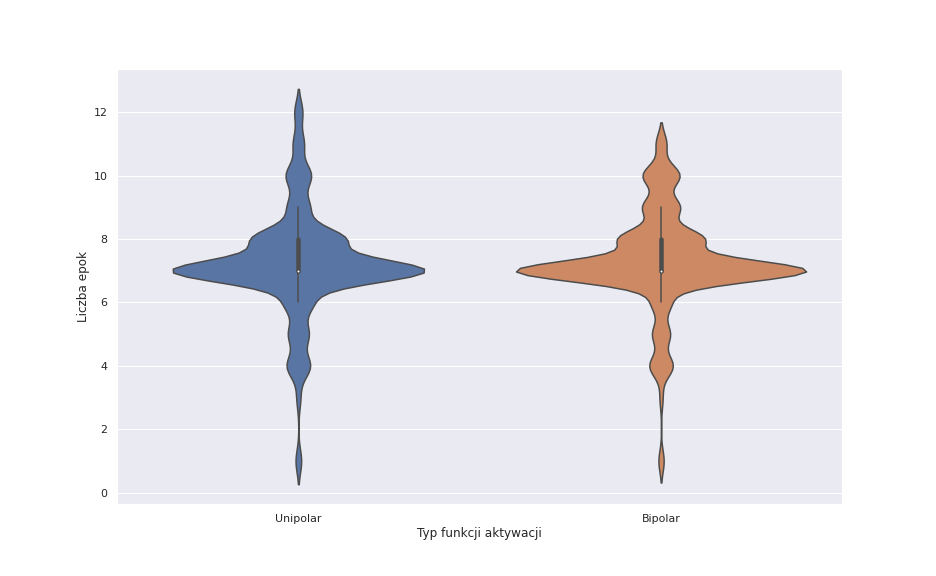
\includegraphics[width=1\textwidth]{images/05_per_uni_bi.png}
\end{figure}

\FloatBarrier
\subsection {Adaline}

\subsubsection{Inicjalizacja wag}
Podobnie jak w przypadku Perceptronu, wagi zostały zainicjowane z rozkładu jednostajnego.
Algorytm Adaline jest bardziej podatny na skalę wag dobraną podczas inicjalizacji.
W przypadku wag z przedziału $\left(0, 0.25\right]$ potrzeba było zaledwie jednej
epoki do osiągnięcia optimum z zadaną dokładnością.

\begin{figure}[h]
  \caption{Wpływ inicjalizacji wag}
  \centering
    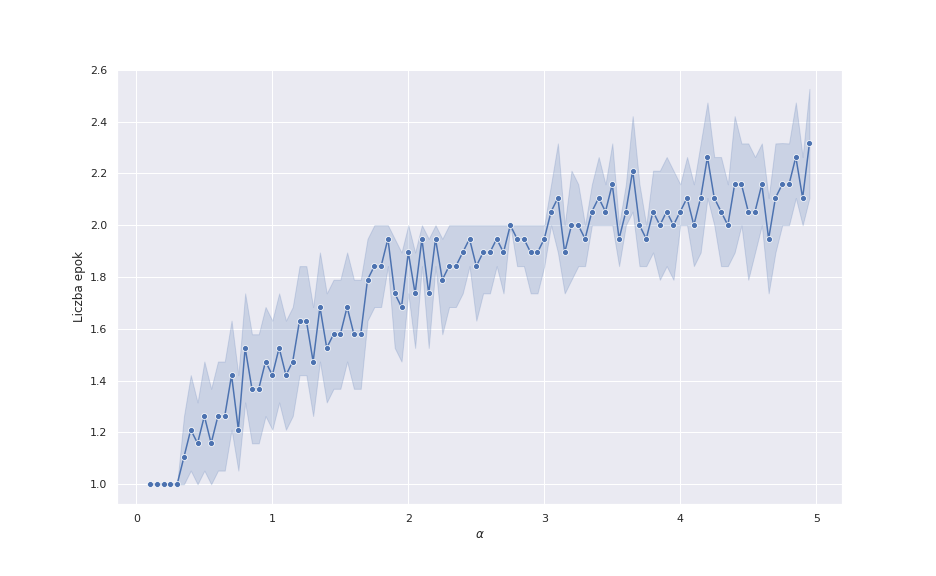
\includegraphics[width=0.8\textwidth]{images/06_ada_interval.png}
\end{figure}

\FloatBarrier
\subsubsection{Współczynnik uczenia $\mu$}
Wpływ współczynnika uczenia okazał się znaczący.
Zbyt małe wartości były powodem wolnego zbiegania do optimum.
Zachowanie funkcji okazało się szczególnie interesujące dla dużych wartości $\mu$.
Ustawienie współczynnika uczenia większego od 0.01 spowodowało eksplozję gradientów, która uniemożliwiła poprawną optymalizację.
Problem zanikających lub eksplodujących gradientów dotyczy szczególnie głębokich sieci neuronowych.
Rozwiązaniem jest dobór odpowiedniej wartości $\mu$ oraz specjalne metody inicjalizacji wag.


\begin{figure}[h]
  \caption{Wpływ $\mu$}
  \centering
    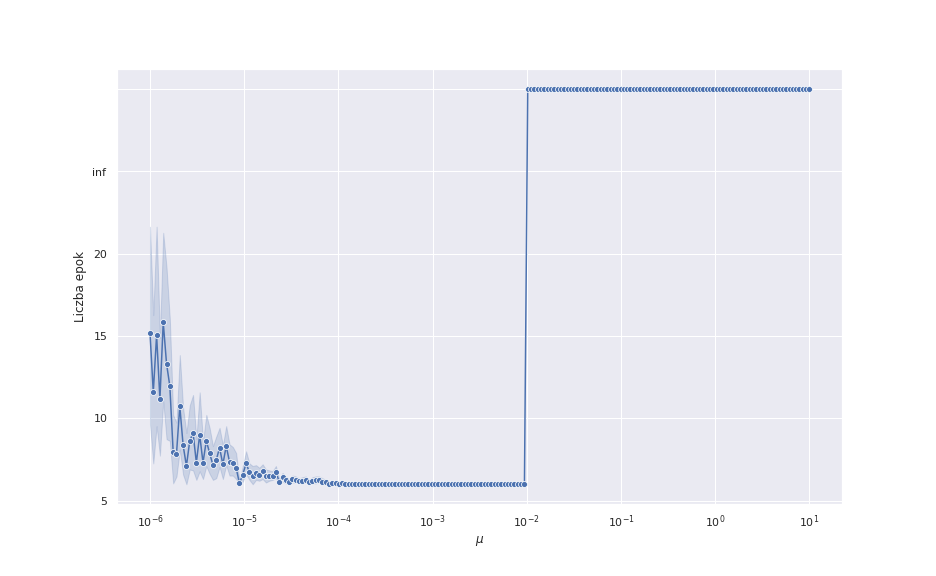
\includegraphics[width=0.8\textwidth]{images/07_ada_lr.png}
\end{figure}
\FloatBarrier

\section{Porównanie Perceptronu i Adaline}
Podstawową różnicą między tymi dwoma modelami jest sposób aktualizacji wag.
W przypadku Perceptronu aktualizacja odbywa się przy pomocy klas, podczas gdy Adaline używa gradientu funkcji błędu.
Intuicyjnie, używanie pochodnej umożliwia określenia, nie tylko czy model popełnił błąd, ale także jak duży był błąd
i jak należy zmienić wagi aby go zminimalizować.
Dodatkowo, należy pamiętać o tym, że wyjście Perceptronu jest wartością dyskretną w przeciwieństwie do Adaline, którego wyjścia są ciągłe.

\subsection{Szybkość zbiegania}
Porównano liczbę epok potrzebnych do wyuczenie obu modeli.
Eksperyment przeprowadzono dla 100 wartości parametrów uczenia z przedziału $\left[10^{-4}, 10^{2}\right]$.
Dla każdej wartości obliczenia powtórzono 10 razy.
Porównanie obu algorytmów może sprawiać trudność, ponieważ różnią się one warunkiem kończącym.
W przypadku Perceptronu zatrzymanie następuje w momencie, w którym wszystkie przykłady zostały poprawnie zaklasyfikowane.
W przypadku Adaline, warunkiem końcowym jest osiągniecie odpowiednio niskiej
wartości funkcji błędu.
Z tego powodu zmodyfikowano Adaline, tak aby reguła zatrzymania odpowiadała regule Perceptronu. 
Z przeprowadzonych eksperymentów wynika, że algorytm Adaline był w stanie osiągnąć wynik zbliżony do perceptronu tylko pod warunkiem ustawienia odpowiednio wysokiego współczynnika uczenia.
Perceptron okazał się być znacznie mniej podatny na zły dobór tego hiperparametru.

\begin{figure}[h]
  \caption{Porównanie Perceptronu i Adaline}
  \centering
    \includegraphics[width=0.8\textwidth]{images/08_per_vs_ada.png}
\end{figure}

\FloatBarrier

\newpage
\section{Wnioski}
Zadaniem obu algorytmów była klasyfikacja binarna klas separowalnych liniowo.
W przypadku bardzo prostego problemu jakim jest symulacja funkcji logicznej AND
oba algorytmy są w stanie osiągnąć optimum w podobnym czasie.
Dla tak prostego problemu Perceptron wydaje się być lepszym wyborem, ze względu na większą stabilność.
Dla bardziej skomplikowanych zadań przewaga Adaline powinna się powiększać,
ponieważ wykorzystywana jest dodatkowa informacja w postaci gradientu błędu,
która pozwala na bardziej efektywną aktualizację wag.

\begin{figure}[h]
  \caption{Granica decyzyjna}
  \centering
    \includegraphics[width=0.8\textwidth]{images/09_decision_border.png}
\end{figure}

\end{document}

Poni¿ej znajduje siê tabela, w której znajduj¹ siê informacje jak zapisaæ poprawnie polskie znaki w formie zakodowanej:
POLSKA LITERA   KOD TEX POLSKA LITERA   KOD TEX
¹       \k{a}   ¥       \k{A}
æ       \'c     Æ       \'C
ê       \k{e}   Ê       \k{E}
³       \l{}    £       \L{}
ñ       \'n     Ñ       \'N
ó       \'o     Ó       \'O
œ       \'s     Œ       \'S
¿       \.z     ¯       \.Z
Ÿ       \'z            \'Z

